\chapter{Längenmetriken}

\section{Graphen}

\begin{definition}[Graph]
  \label{def:graph}
  Ein \term{Graph} $ G = (E, K) $ besteht aus einer \emph{Ecken}-Menge $ E $ und einer Menge von Paaren $ \{ u, v \} $ ($ u, v \in E $), genannt \emph{Kanten}.
\end{definition}

\begin{definition}[Erreichbarkeit]
  Seien $ p, q \in E $ von $ G = (E, K) $. $ q $ ist \term{erreichbar} von $ p $ aus, falls ein \emph{Kantenzug} von $ p $ nach $ q $ existiert.
\end{definition}

\begin{definition}[Zusammenhängend]
  $ G = (E, K) $ heißt \term{zusammenhängend}, falls alle Ecken von einer beliebigen, festen Ecke aus erreichbar sind.
  \\
  Ist $ G $ ein zusammenhängender \hyperref[def:graph]{Graph}, so ist $ d(p, q) = $ minimale Kantenzahl eines Kantenzuges von $ p $ nach $ q $ eine \hyperref[def:metrik]{Metrik}.
\end{definition}

\begin{example}[Wortmetrik]
  Sei $ \Gamma \coloneqq \langle S \rangle $ vom endlichen Erzeugendensystem $ S $ erzeugte Gruppe. Dann:
  \begin{equation}
    \label{gl:wortmetrik}
    g \in \Gamma \Rightarrow g = s_1\cdot \dots s_n\text{ (multiplikativ, nicht eindeutig),}
  \end{equation}
  z.B. $ \Z = \langle \pm 1 \rangle $. \\
  Dann lässt sich über die Länge von $ g \in \Gamma $ (minimales $ n $ in \autoref{gl:wortmetrik}) eine \hyperref[def:metrik]{Metrik} definieren:
\end{example}

\begin{definition}[Wortmetrik]
  \label{def:wortmetrik}
  \begin{equation*}
    d_S(g, k) \coloneqq |g^{-1}k|
  \end{equation*}
  ist eine \hyperref[def:metrik]{Metrik} mit
  \begin{align*}
    d_s(kg,kh) &= |(kg)^{-1}kh| \\ 
    &= |g^{-1}\underbrace{k^{-1}k}_{=e}h| = |g^{-1}h| \\
    &= d_s(g,h)\text{,}
  \end{align*}
  also ist $ d_s $ linksmultiplikativ mit $ k \in \Gamma $ und damit eine \hyperref[def:isometrie]{Isometrie}.
\end{definition}

\begin{definition}[Cayley-Graph]
  Der \term{Cayley-Graph} $ \text{Cay}(\Gamma, S) $ von $ \Gamma $ bezüglich $ S $ ist der Graph $ G = (E, K) $ mit
  \begin{equation*}
    E \coloneqq \Gamma, \quad K \coloneqq \{ (g, gs) : g \in \Gamma, s \in S \}\text{.}
  \end{equation*}
  Die \emph{Graphen-Metrik} auf $ \text{Cay}(\Gamma, S) $ ist \hyperref[def:isometrie]{isometrisch} zur \hyperref[def:wortmetrik]{Wortmetrik}.
\end{definition}

\section{Euklidische Metrik}
\begin{example}[Euklidische Metrik auf $ \R^2 $ als Standardmetrik]
  Sei
  \begin{equation*}
    c : [a,b] \to \R^2, \quad t \mapsto (x(t), y(t))
  \end{equation*}
  eine stückweise differenzierbare\footnote{\textbf{Hinweis}: Mit \emph{differenzierbar} ist im Folgenden immer $ C^\infty $-differenzierbar gemeint, wenn nicht anders angegeben.} Kurve.
  Die \emph{euklidische Länge} von $ C $ ist
  \begin{align*}
    L_{\text{euk}}(c) &\coloneqq \int_a^b \Vert C'(t) \Vert dt \quad \text{(via \emph{Polynom-Approximation})} \\
     &= \int_a^b \sqrt{\left( x'(t) \right)^2 + \left( y'(t) \right)^2}dt\text{.}
  \end{align*}
  \begin{figure}[H]
    \label{img006-1}
    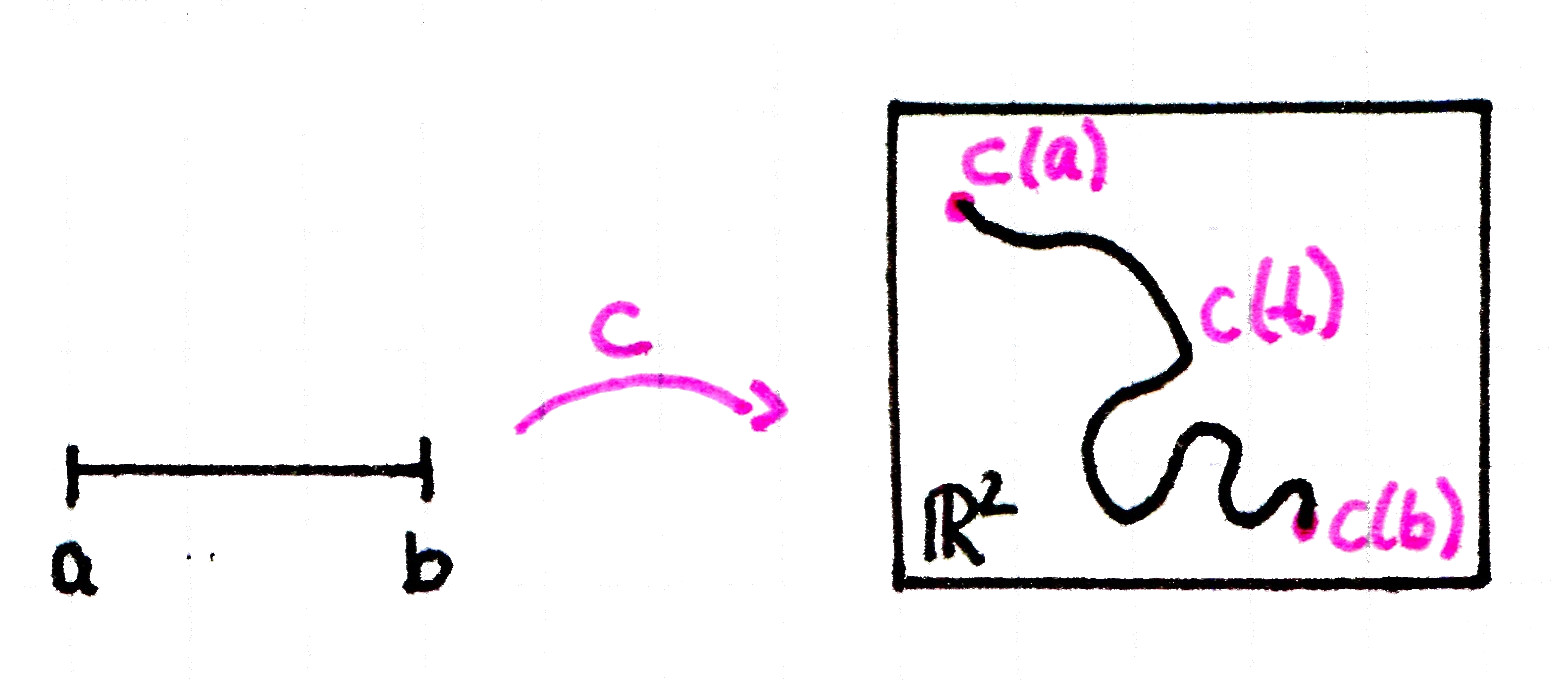
\includegraphics[width=.5\textwidth]{img006-1}
    \caption{Eine stückweise differenzierbare Kurve im $ \R^2 $}
  \end{figure}
  \emph{Beispiel}: Geraden-Segment.
  \begin{equation*}
    g: [0,1] \to \R^2, \quad t \mapsto g(t) = (1-t)p + tq\text{.}
  \end{equation*}
  Dann:
  \begin{equation*}
    g'(t) = -p+q, \quad \Vert g'(t) \Vert = \Vert p - q \Vert
  \end{equation*}
  und damit
  \begin{equation*}
    \underline{L_{\text{euk}}(g)} = \int_0^1\Vert p - q \Vert dt = \Vert p - q \Vert = \underline{d_e(p,q)}\text{.}
  \end{equation*}
\end{example}

\begin{lemma}[Unabhängigkeit von $ \text{L}_\text{euk} $]
  \label{lm:leuklinvarianz} \
  \begin{enumerate}
    \item $ L_\text{euk}(c) $ ist unabhängig von Kurvenparametrisierung.
    \item $ L_\text{euk}(c) $ ist invariant unter Translationen, Drehungen und Spiegelungen.
  \end{enumerate}
  \begin{proof}
    \
    \begin{enumerate}
      \item Zu zeigen: Für $ c: [a,b] \to \R^2 $, $ t \mapsto c(t) $ und einen monoton wachsenden Diffeomorphismus\footnote{\textbf{Diffeomorphismus}: Bijektive, stetig differenzierbare Abbildung, deren Umkehrabbildung auch stetig differenzierbar ist.} $ t: [c, d] \to [a,b] $, $ s \mapsto t(s) $ gilt:
      \begin{equation*}
        L_\text{euk}(c(t(s))) = L_\text{euk}(c(t))\text{.}
      \end{equation*}
      Das folgt unmittelbar aus der Substitutionsregel für Integrale:
      \begin{equation*}
        \int_c^d \left\Vert \frac{dc}{ds} \right\Vert ds = \int_c^d \left\Vert \frac{d_c(t(s))}{dt} \right\Vert \frac{dt}{ds}ds = \int_{t(c) = a}^{t(d)=b} \left\Vert \frac{dc}{dt} \right\Vert dt \text{.}
      \end{equation*}\qed
      \item \begin{itemize}
        \item \underline{Translation}. \\ Für $ p = (p_1, \dots, p_n) \in \R^2 $ sei
        \begin{equation*}
           T_p(c(t)) = c(t) + p = (\lambda(t) + p_1, y(t) + p_2)
         \end{equation*} 
         die von $ p $ verschobene Kurve. Es gilt
         \begin{equation*}
           (T_p \circ c)(t) = c'(t) \Rightarrow \int_a^b \left\Vert (T_p \circ c)' \right\Vert dt = \int_a^b \left\Vert c' \right\Vert dt
         \end{equation*}
         und damit gilt das Lemma für Translationen. \qed
        \item \underline{Drehung}. \\
        Für $ \theta \in [0,2\pi] $ sei
        \begin{align*}
          D_\theta \circ c(t) &= \begin{pmatrix}
            \cos\theta & -\sin\theta \\
            \sin\theta & \cos\theta
          \end{pmatrix}c(t) \\ 
           &= (\cos\theta x(t) - \sin\theta y(t), \sin\theta x(t) + \cos\theta y(t))
        \end{align*}
        die um Winkel $ \theta $ gedrehte Kurve. \\
        Da $ D_\theta $ eine orthogonale Abbildung ist, folgt
        \begin{equation*}
          (D_\theta \circ c(t))' = D_\theta * c'(t)
        \end{equation*}
        und damit
        \begin{equation*}
          \left\Vert (D_\theta \circ c(t))' \right\Vert = \left\Vert D_\theta * c' \right\Vert \overset{\text{orth.}}{=} \left\Vert c' \right\Vert
        \end{equation*}
        und damit gilt das Lemma für Drehungen. \qed
        \item Spiegelungen sind wie Drehungen orthogonal, ihre Invarianz folgt aus der Invarianz der Drehungen.
      \end{itemize}
    \end{enumerate}
  \end{proof}
\end{lemma}

\begin{lemma}[Geraden sind am kürzesten]
  \label{lemma:geradenkurz}
  Die kürzesten Verbindungskurven zwischen Punkten in $ \R^2 $ sind genau die Geradensegmente. \\
  \begin{proof}
    \ \\
    \begin{minipage}{.45\textwidth}
      Seien $ p, q \in \R^2 $ beliebig. Durch geeignete Rotation und Translation kann man $ (p,q) $ überführen in Punkte in spezieller Lage;
      \begin{equation*}
        p' = (0,0), \quad q' = (0,l)\text{.}
      \end{equation*}
      Wegen \hyperref[lm:leuklinvarianz]{der Invarianz von $ L_\text{euk} $} ändert sich dabei die Länge entsprechender Verbindungskurven nicht. \\
      Sei jetzt $ c(t) \coloneqq (x(t),y(t)) $ eine stückweise differenzierbare Kurve zwischen $ p' $ und $ q' $. Dann gilt:
    \end{minipage}
    \hfill
    \begin{minipage}{.45\textwidth}
      \begin{figure}[H]
        \label{img007-1}
        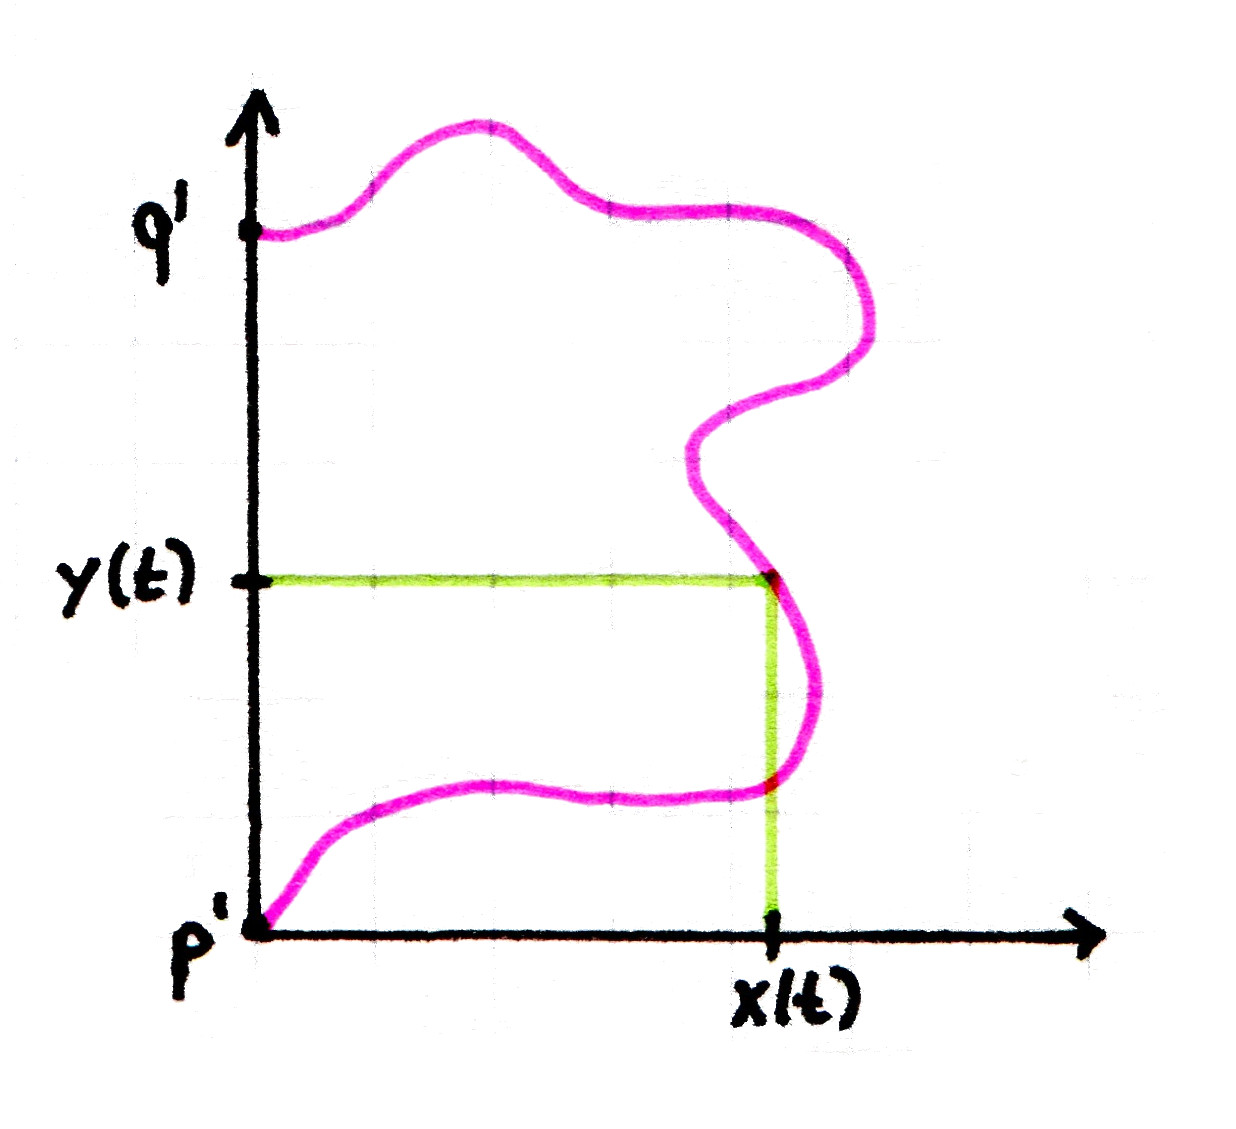
\includegraphics[width=.8\textwidth]{img007-1}
        \caption{Die ``geeignete'' Rotation einer Kurve, sodass Start- und Endpunkt auf einer Achse liegen}
      \end{figure}
    \end{minipage}
    \begin{align*}
      L_\text{euk}(c) &= \int_a^b\sqrt{(x')^2+(y')^2}dt \geq \int_a^b\vert y' \vert dt \geq \int_a^by'(t)dt = \int_{y(a) = 0}^{y(b) = l} dy \\
       &= l\text{.}
    \end{align*}
    $ l $ ist die Länge des Geradensegmentes zwischen $ p' $ und $ q' $. \\
    $ \Rightarrow $ \underline{Infimum} der Längenwerte wird angenommen. Eindeutigkeit bleibt zu zeigen. \\
    Gilt für eine Kurve $ c $, dass $ L_\text{euk}(c) = l $, so hat man in obigen Ungleichungen überall Gleichheit, also insbesondere $ x'(t) = 0 $ ($ \forall t $), also $ x(t) = \text{konstant} = x(0) = 0 $ und somit $ \widetilde{c} = (0,y(t)) $. Also ist $ \widetilde{c} $ auch (parametrisiertes) Geradensegment. \qed
  \end{proof}
\end{lemma}

\begin{definition}[Euklidische Metrik auf $ \R^2 $-Kurven]
  Für $ p,q \in \R^2 $ sei $ \Omega_{pq}(\R^2) $ die Menge der stetig differenzierbaren Verbindungskurven zwischen $ p $ und $ q $. Wir setzen dann:
  \begin{equation*}
    (p,q) = \inf L_\text{euk}(c), \quad c \in \Omega_{pq}(\R^2)\text{.}
  \end{equation*}
\end{definition}

\begin{theorem}[``Neuer'' \ metrischer $ \R^2 $]
  \begin{equation*}
    (\R^2, d_\text{euk})
  \end{equation*}
  ist ein \hyperref[def:metrischerRaum]{metrischer Raum} und \hyperref[def:isometrie]{isometrisch} zu $ (\R^2, d_e) $.
  \begin{proof}
    Direkter Beweis nach dem \hyperref[lemma:geradenkurz]{Lemma über Geradensegmente}. \\
    Man hat eine explizite Formel
    \begin{equation*}
      d_{\text{euk}}(p,q) = \Vert p - q \Vert = d_e(p,q)\text{.}
    \end{equation*}
    Die Identität ist eine Isometrie.
  \end{proof}
  \begin{proof}
    Konzeptioneller, allgemeinerer Beweis. Es werden die Metrik-Eigenschaften gezeigt.

    \begin{itemize}
      \item \emph{Symmetrie}. \\
        Sei
        \begin{equation*}
          \Omega_{pq}(\R^2) \ni c: [a,b] \to \R^2\text{.}
       \end{equation*}
       Idee: Kurve wird rückwärts durchlaufen. \\
       Es ist $ d_\text{e} = d_\text{euk} $, denn ist $ \widetilde{c}(t) = (a+b-t) \in \Omega_{qp}(\R^2) $ (mit gleicher Länge wie $ c $) und die Abbildung $ c \mapsto \widetilde{c} $ ist bijektiv. Dann $ L(\widetilde{c}) = L(c) $, und damit
       \begin{equation*}
         d(q,p) = \inf(L(\widetilde{c})) = \inf(L(c)) = d(p,q)\text{.}
       \end{equation*}

      \begin{minipage}{.45\textwidth}
        \item \emph{Dreiecksungleichung}. \\
          Zu zeigen: $ d_\text{euk}(p,q) \leq d_\text{euk}(p,r) + d_\text{euk}(r,q) $ ($ \forall p, q, r \in \R^2 $). \\
          Verknüpfen von Wegen von $ p $ nach $ r $ mit solchen von $ r $ nach $ q $ liefert gewisse --- aber i.A. nicht alle --- Wege von $ p $ nach $ q $:
          \begin{equation*}
            \Omega_{pr} \cup \Omega_{rq} \subsetneq \Omega_{pq}\text{.}
          \end{equation*}
          Infimumbildung liefert die Behauptung.
      \end{minipage}
      \hfill
      \begin{minipage}{.45\textwidth}
        \begin{figure}[H]
          \label{img008-1}
          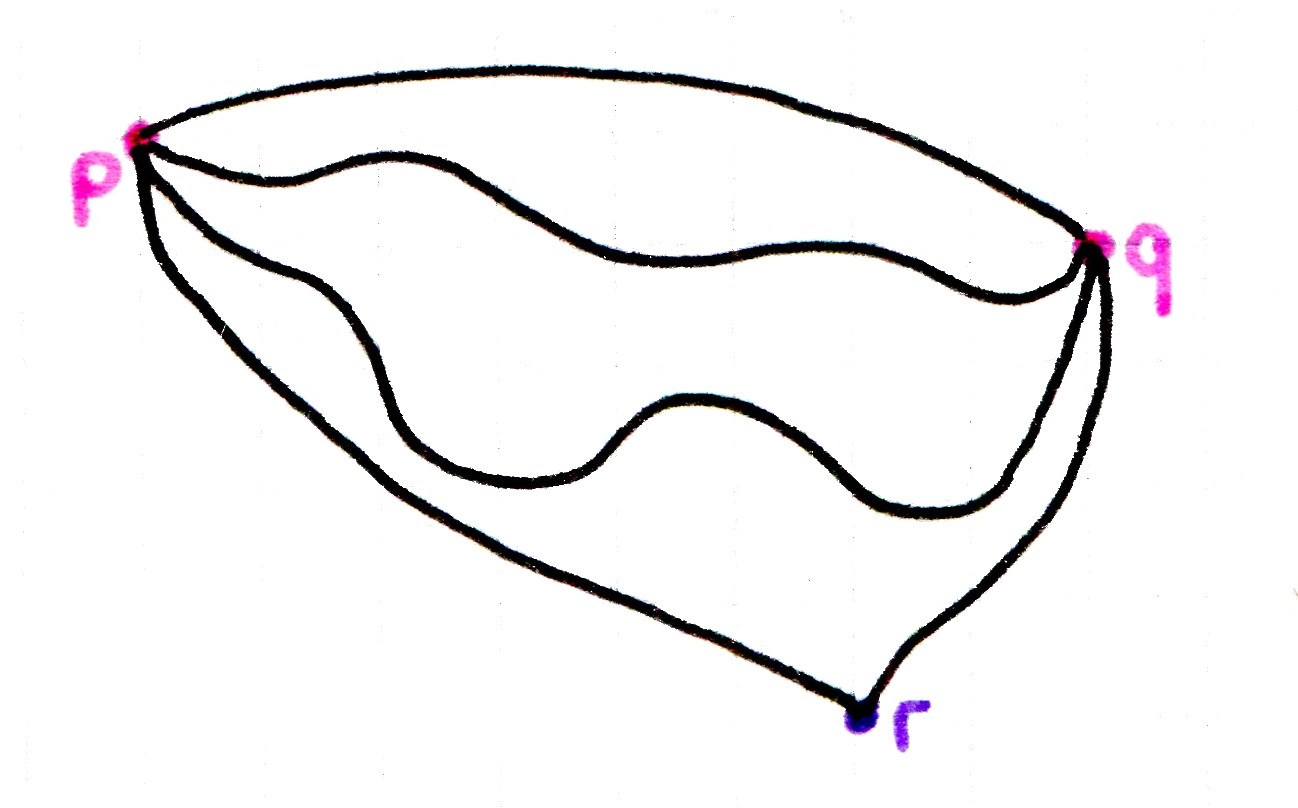
\includegraphics[width=.8\textwidth]{img008-1}
          \caption{Betrachte Wege von $ p $ nach $ q $ über $ r $ und nicht über $ r $}
        \end{figure}
      \end{minipage}

      \begin{minipage}{.45\textwidth}
        \item \emph{Positivität}. \\
          Zu zeigen: $ d_\text{euk}(p,q) = 0 \Leftrightarrow p = q $.
          \begin{itemize}
            \item Falls $ p = q $. \\
              Die konstante Kurve $ c: [0,1] \to \R^2, t \mapsto c(t) = p $ hat 
              \begin{equation*}
                c'(t) = 0 \Rightarrow L_\text{euk}(c) = 0 \leadsto d_\text{euk}(p,p) = 0 \text{.}
              \end{equation*}
            \item Falls $ p \neq q $. \\
              Die kürzeste Kurve ist das Geradensegment\footnotemark
              \begin{equation*}
                t \mapsto (1-t)p + tq
              \end{equation*}
              mit der Länge $ d_\text{euk} = \Vert p - q \Vert = 0 $.
          \end{itemize}
      \end{minipage}
      \footnotetext{\textbf{Anmerkung}: nur an dieser Stelle wird die Geometrie des $ \R^2 $ benötigt!}
      \hfill
      \begin{minipage}{.45\textwidth}
        \begin{figure}[H]
          \label{img008-1}
          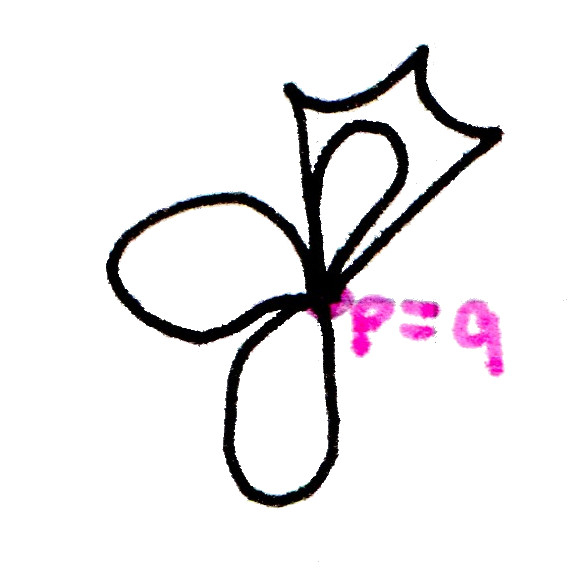
\includegraphics[width=.5\textwidth]{img008-2}
          \caption{``Schleifen''}
        \end{figure}
      \end{minipage}
    \end{itemize}
  \end{proof}
\end{theorem}

\section{Sphärische Geometrie}
\begin{example}[2-dimensionale sphärische Geometrie als Längenraum]
  Eine $ 2 $-dimensionale Sphäre von Radius $ R $ in $ \R^3 $ ist
  \begin{equation*}
    S^2_R \coloneqq \{ x \in \R^3 : \Vert x \Vert = R \} = \{ (x_1, x_2, x_3) \in \R^3 : x_1^2+x_2^2+x_3^2 = R^2 \}\text{.}
  \end{equation*}
  \begin{minipage}{.65\textwidth}
  Für eine stückweise differenzierbare Kurve
    \begin{equation*}
      c: [a,b] \to S^2_R \subset \R^3, \ t \mapsto (x_1(t), x_2(t), x_3(t))
    \end{equation*}
    definiere die \term{sphärische Länge} durch
    \begin{equation*}
      L_S(c) \coloneqq \int_a^b \Vert c'(t) \Vert dt = \int_a^b \sqrt{{x'}_1^2+{x'}_2^2+{x'}_3^2}dt
    \end{equation*}
    und
    \begin{equation*}
      d_s(p,q) \coloneqq \inf L_s(c) \quad (c \in \Omega_{pq}(S^2_R))\text{.}
    \end{equation*}
  \end{minipage}
  \hfill
  \begin{minipage}{.25\textwidth}
    \begin{figure}[H]
      \label{img009-1}
      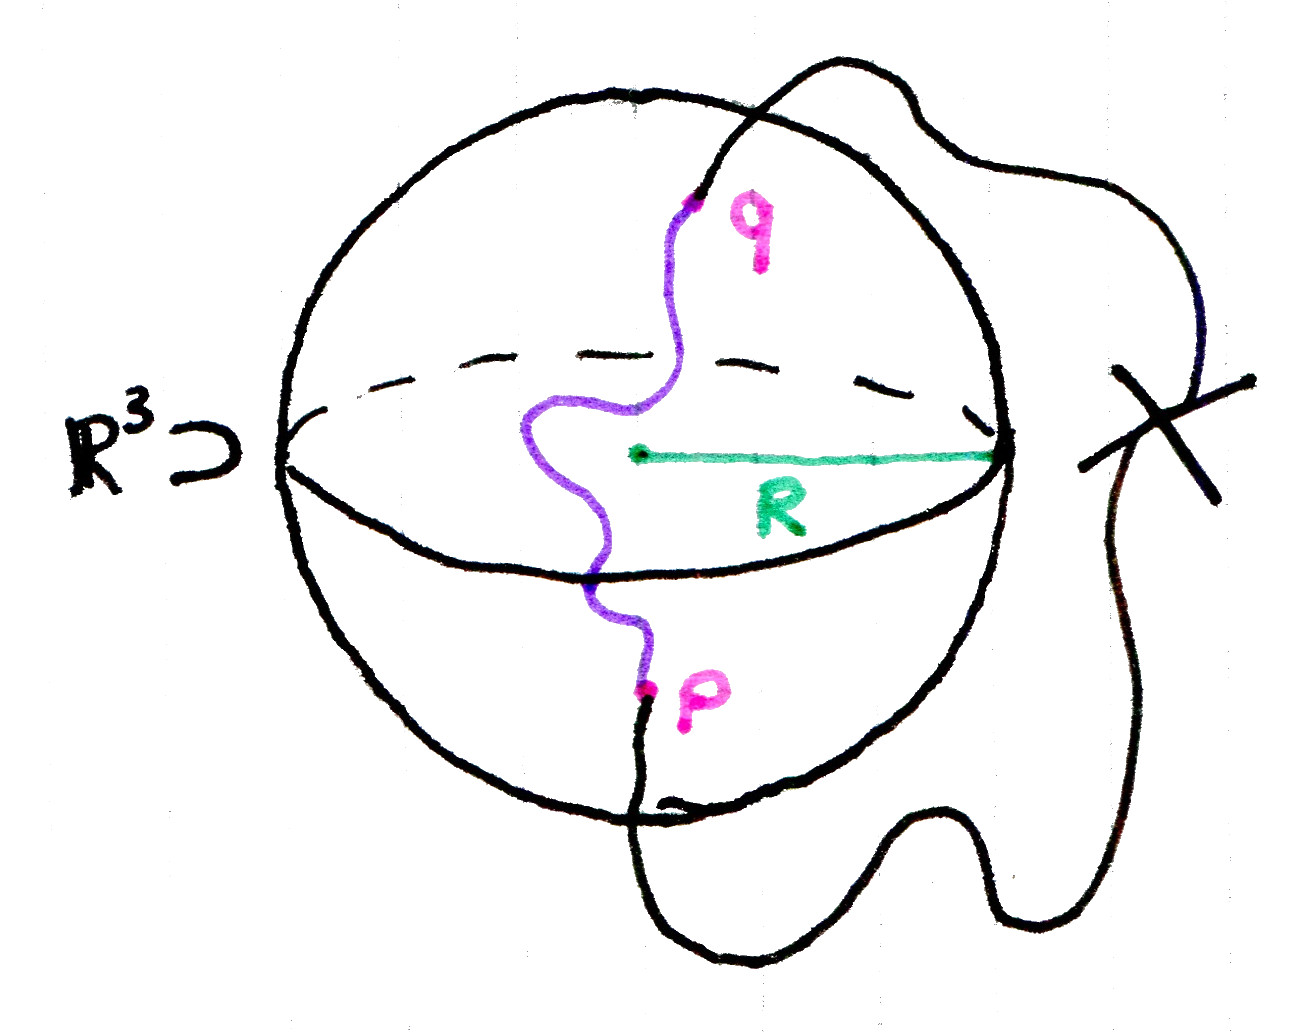
\includegraphics[width=\textwidth]{img009-1}
      \caption{Es werden nur Kurven betrachtet, die \underline{in} $ S_R^2 $ liegen}
    \end{figure}
  \end{minipage}
\end{example}

\begin{lemma}[Kurvenlängen rotationsinvariant]
  \label{lemma:kurvenlaengen}
  Die Länge einer differenzierbaren Kurve auf $ S^2_R $ ist invariant unter Rotationen von $ \R^2 $.
  \begin{proof}
    Eine orthogonale Matrix im $ \R^2 $ ist (bzgl. Standardbasis) gegeben durch eine orthogonale Matrix $ D \in \R^{2 \times 2} $. Da $ \Vert D(x) \Vert = \Vert x \Vert $ für $ x \in \R^3 $ gilt, ist $ D(S^2_R) = S^2_R $. Insbesondere ist für eine Kurve $ c $ in $ S^2_R $ auch das Bild $ D \circ c \subset S^2_R $. \\
    Weiter folgt aus $ (D \circ c(t))' = D \circ c'(t) $:
    \begin{align*}
      L_s(D \circ c) &= \int_a^b \Vert (D \circ c(t))' \Vert dt = \int_a^b \Vert D(c'(t)) \Vert dt \\
        &= \int_a^b \Vert c'(t) \Vert dt = L_S(c)\text{.}
    \end{align*}
  \end{proof}
\end{lemma}

\begin{lemma}[Großkreise sind am kürzesten]
  \ \\
  \begin{minipage}{.45\textwidth}
    Die kürzesten Verbindungskurven zwischen zwei Punkten in $ S^2_R $ sind \term{Großkreise}, also Schnitte von $ S^2_R $ und zweidimensionalen Untervektorräumen des $ \R^3 $.
  \end{minipage}
  \hfill
  \begin{minipage}{.45\textwidth}
    \begin{figure}[H]
      \label{img009-2}
      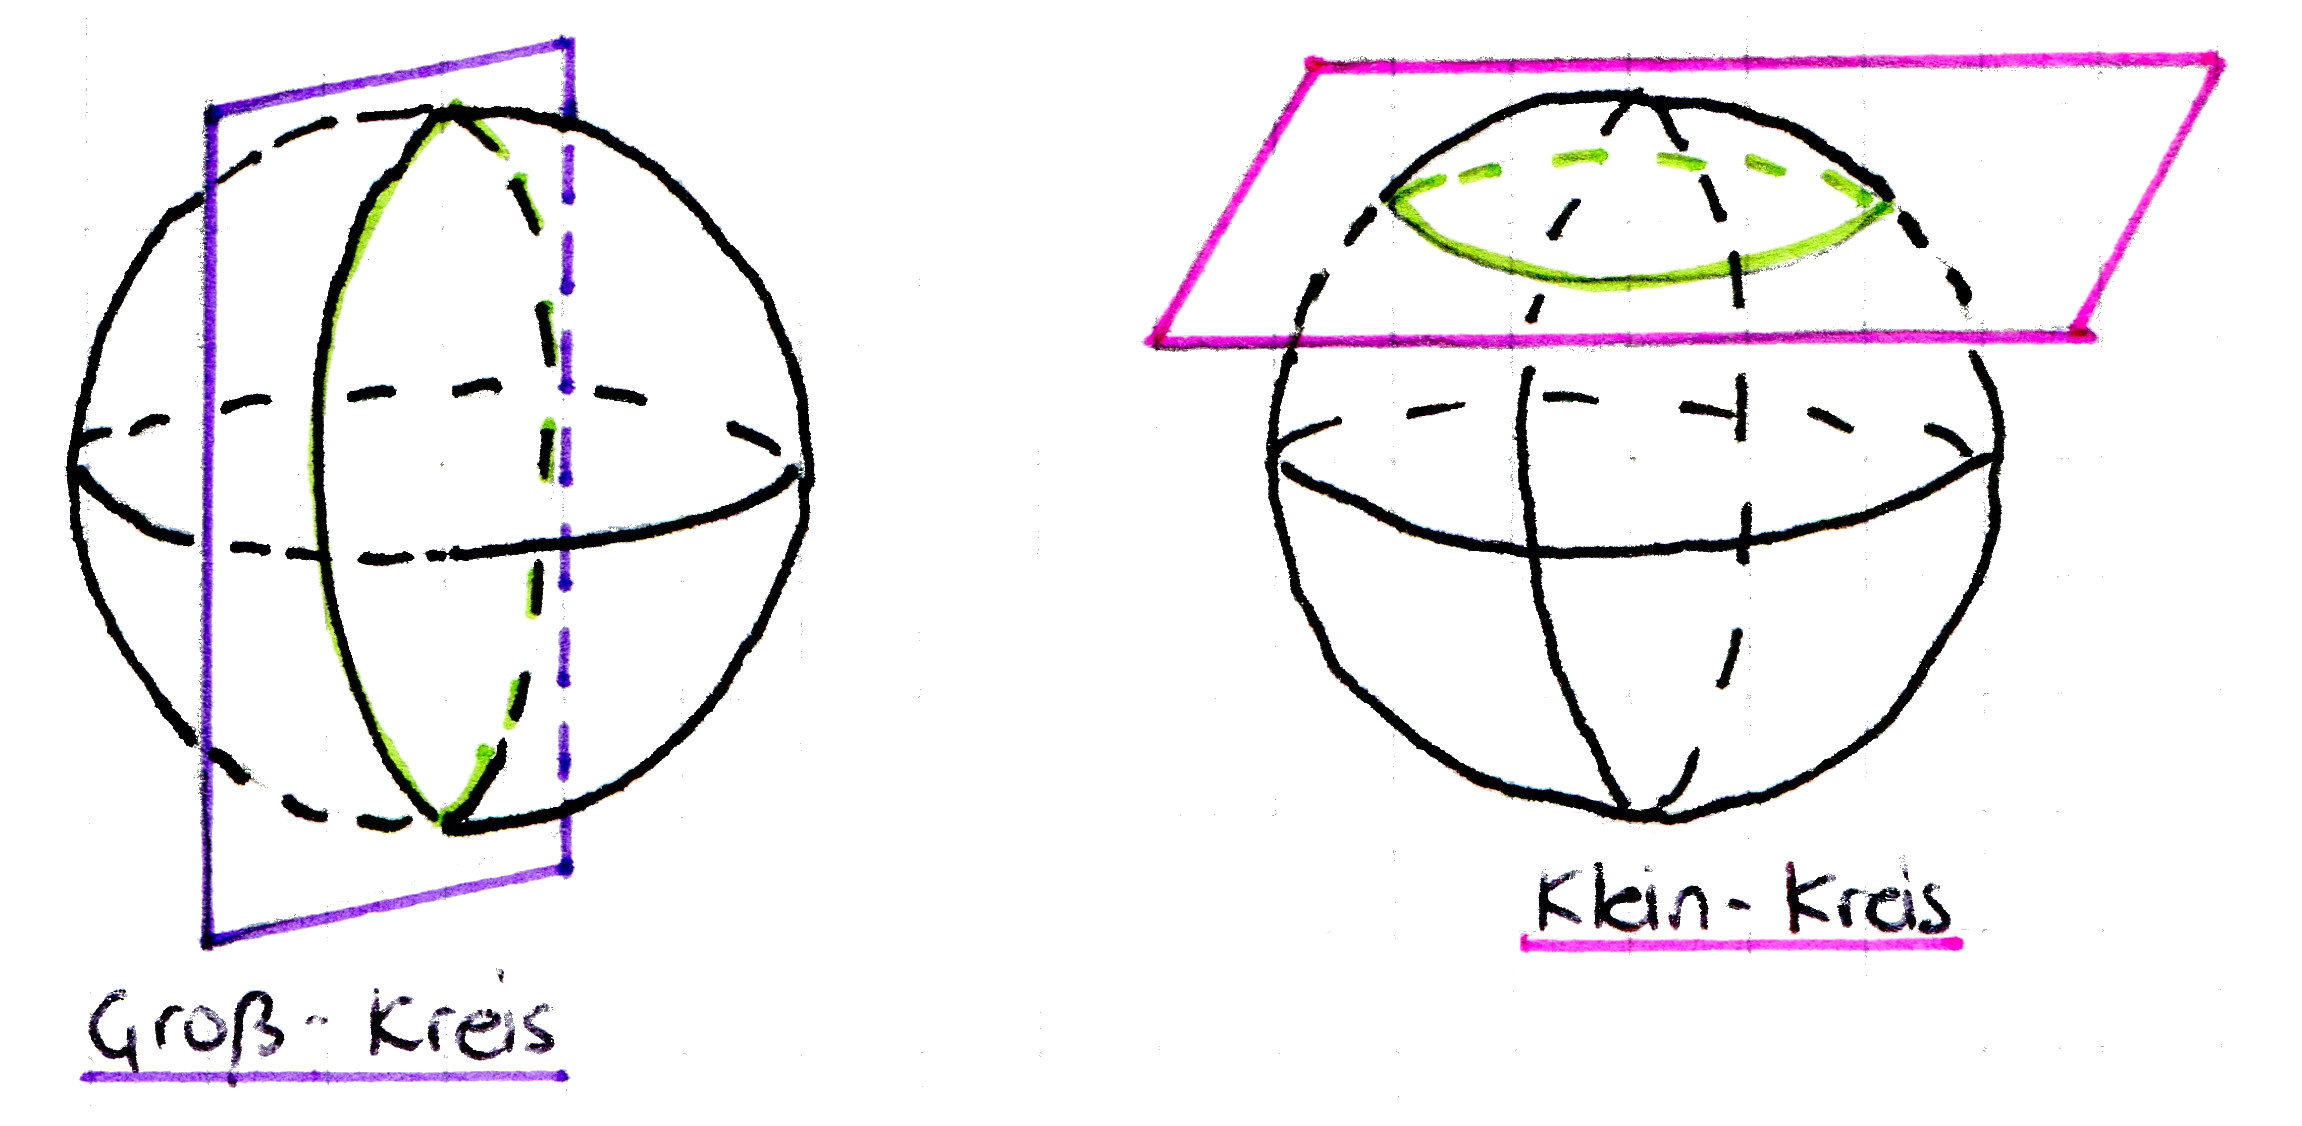
\includegraphics[width=\textwidth]{img009-2}
      \caption{Groß- uund Klein-Kreis}
    \end{figure}
  \end{minipage}
  \begin{proof}
    \ \\
    \begin{minipage}{.45\textwidth}
      Seien zwei beliebige Punkte $ p,q $ auf $ S^2_R $. Dann finden wir eine Rotation von $ \R^3 $, die $ p $ auf $ p' = (0,0,R) $ --- also den ``Nordpol'' --- und $ q $ auf $ q' = (0,y,z) \in S^2_R $ abbildet. Aufgrund der \hyperref[lemma:kurvenlaengen]{Rotationsinvarianz der Kurvenlängen} und der Definition ist $ d_s(p,q) = d_s(p', q') $. Es genügt also eine kürzeste Verbindung zwischen $ p' $ und $ q' $ zu finden. \\
      \emph{Idee}: Mittels ``geographischer Koordinaten'' $ \varphi $ und $ \theta $. Nun kann eine Verbindung zwischen $ p' $ und $ q' $ geschrieben werden als
    \end{minipage}
    \hfill
    \begin{minipage}{.45\textwidth}
      \begin{figure}[H]
        \label{img010-1}
        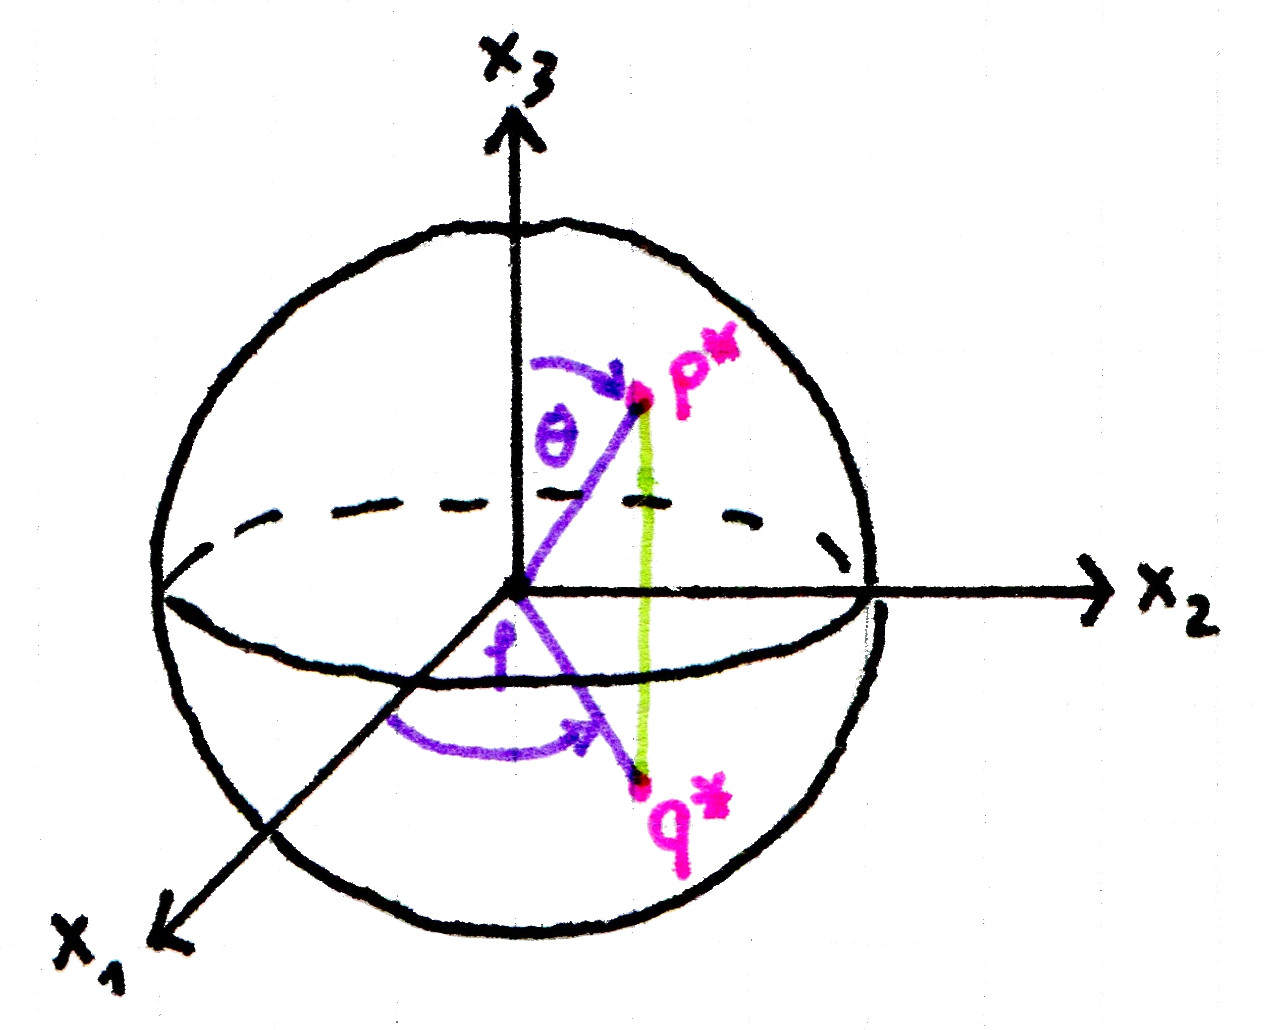
\includegraphics[width=\textwidth]{img010-1}
        \caption{Geographische Koordinaten auf $ S_R^2 $}
      \end{figure}
    \end{minipage}
    \begin{equation*}
      c(t) = R(\sin\theta(t)\cos\varphi(t), \ \sin\theta(t)\sin\varphi(t), \ \cos\theta(t))
    \end{equation*}
    und somit
    \begin{small}
      \begin{equation*}
        c'(t) = (\theta'\cos\theta\cos\varphi-\varphi'\sin\theta\sin\varphi, \ \theta'\cos\theta\sin\varphi+\varphi'\sin\theta\cos\varphi, \ -\theta'\sin\theta)\text{,}
      \end{equation*}
    \end{small}
    also
    \begin{equation*}
      \Vert c'(t) \Vert = R^2({\theta'}^2 + {\varphi'}^2\sin^2\theta)
    \end{equation*}
    und somit
    \begin{align*}
      L_s(c) &= R\int_a^b\sqrt{{\theta'}^2+{\varphi'}^2\sin^2\theta}dt \geq R\int_a^b\sqrt{{\theta'}^2(t)}dt \\
      &= R\int_a^b \vert \theta'(t) \vert dt \geq R\int_a^b \theta'(t)dt = \int_{\theta(a)}^{\theta(b)}d\theta = R(\theta(b)-\theta(a))
    \end{align*}
    mit oBdA $ \theta(b) \geq \theta(a) $. \\
    Diese untere Schranke wird durch ein Großkreissegment realisiert. \\
    Eine weitere Kurve diese Länge kann es (wieder) nicht geben --- man hätte sonst überall Gleichheit in den Ungleichungen, also insbesondere $ \varphi' = 0 $, also wäre $ \varphi $ konstant $ = \varphi(a) = \frac{\pi}{2} $. Also liegt die Kurve auf Meridian und ist somit Großkreis.
  \end{proof}
\end{lemma}

\begin{theorem}[Infimums- \& Winkelmetrik isometrisch]
  $ (S^2_R, d_s) $ ist ein metrischer Raum und isometrisch zu $ (S^2_R, R*d_W) $.
  \begin{proof}
    Analog zu $ (R^2, d_\text{euk}) $.
  \end{proof}
\end{theorem}

\section{Wozu sind Metriken gut?}

\begin{remark}[Erinnerung: Konvergenz]
  In Analysis I heißt eine Folge von reellen Zahlen $ (a_n)_{n \in \N} $ \emph{konvergent}, wenn
  \begin{equation*}
    \exists \ a \in \R : \forall \epsilon > 0 \ \exists \ N = N(\epsilon) : \vert a_n - a \vert < \epsilon \quad (\forall n \geq N)\text{.}
  \end{equation*}
\end{remark}

\begin{remark}[Konvergenz in metrischen Räumen]
  Sei $ (X, d) $ metrischer Raum. \\
  Eine Folge $ (x_n)_{n \in \N} $ aus $ X $ heißt \term{konvergent}, wenn
  \begin{equation*}
    \exists \ x \in X \forall \epsilon > 0 \ \exists \ N = N(\epsilon) : d(x_n, x) \leq \epsilon \quad (\forall n \geq N)\text{.}
  \end{equation*}
  Also $ x_n \in B_\epsilon(x) $ ($ \forall n \geq N $).
\end{remark}

\begin{remark}[Erinnerung: Stetigkeit]
  $ f: \R \to \R $ heißt \emph{stetig} in $ t_0 \in \R $ falls
  \begin{equation*}
    \forall \epsilon > 0 \ \exists \ \delta = \delta(\epsilon) > 0 : \vert t - t_0 \vert < \delta \Rightarrow \vert f(t)-f(t_0) \vert < \epsilon\text{.}
  \end{equation*}
  $ f $ heißt \emph{stetig}, wenn sie stetig ist $ \forall t_0 \in \R $.
\end{remark}

\begin{remark}[Stetigkeit in metrischen Räumen]
  Metrische Räume $ (X, d_X), \ (Y, d_Y) $. \\
  Eine Abbildung $ f: X \to Y $ heißt \term{stetig} in $ x_0 \in X $, falls
  \begin{equation*}
    \forall \epsilon > 0 \ \exists \ \delta = \delta(\epsilon) > 0
  \end{equation*}
  sodass
  \begin{equation*}
    d_Y(f(x), f(x_0)) < \epsilon \text{ falls } d_X(x, x_0) < \delta\text{.}
  \end{equation*}
  Also wenn $ f(x) \in B_\epsilon^Y(f(x)) $ falls $ x \in B_\delta^X(x_0) $. \\
  $ f $ heißt \emph{stetig}, falls $ f $ stetig ist $ \forall x \in X $.
\end{remark}

\begin{remark}[Grenzwerte für stetige Funktionen]
  \begin{equation*}
    f: X \to Y $ stetig $ \Rightarrow f(\lim_{n \to \infty}x_n) = \lim_{n \to \infty}f(x_n)\text{.}
  \end{equation*}
  Als Übungsaufgabe zu zeigen, der Beweis ist analog zum Beweis in der Analysis. \\
  Diese Beobachtung führt historisch (um 1900) durch die Verallgemeinerung metrischer Räume zu topologischen Räume.
\end{remark}